\documentclass[aspectratio=169]{beamer}
\usetheme{Warsaw}
\usecolortheme{beaver}

\usepackage{listings}
\usepackage{graphicx}
\usepackage{tikz}
\usepackage{amsmath}
\usepackage{amssymb}
\usepackage{algorithm2e}
\usepackage{xcolor}

\usetikzlibrary{shapes,arrows,positioning,calc}

\lstset{
    basicstyle=\tiny\ttfamily,
    keywordstyle=\color{blue},
    commentstyle=\color{green!60!black},
    stringstyle=\color{red},
    breaklines=true,
    showstringspaces=false,
    frame=single,
    language=Python
}

\title{pyHMSSQL: A Complete Database Management System}
\subtitle{Architecture, Theory, and Execution Pipeline}
\author{Database Systems Analysis}
\date{\today}

\begin{document}

\frame{\titlepage}

\begin{frame}{Outline}
\tableofcontents
\end{frame}

\section{Introduction and System Overview}

\begin{frame}{What is pyHMSSQL?}
\begin{itemize}
    \item \textbf{Complete DBMS Implementation} in Python
    \item \textbf{Client-Server Architecture} with socket-based communication
    \item \textbf{Custom B+ Tree Indexing} for efficient data retrieval
    \item \textbf{Full SQL Support} including complex queries, joins, transactions
    \item \textbf{Advanced Features}: Views, stored procedures, triggers, replication
    \item \textbf{Multiple Interfaces}: CLI, GUI (JavaFX), REST API
\end{itemize}

\vspace{0.3cm}
\begin{block}{Key Innovation}
Unlike most academic DBMS projects, pyHMSSQL implements \textbf{production-grade features} including ACID transactions, foreign key constraints, query optimization, and distributed replication.
\end{block}
\end{frame}

\begin{frame}{System Architecture Overview}
\begin{center}
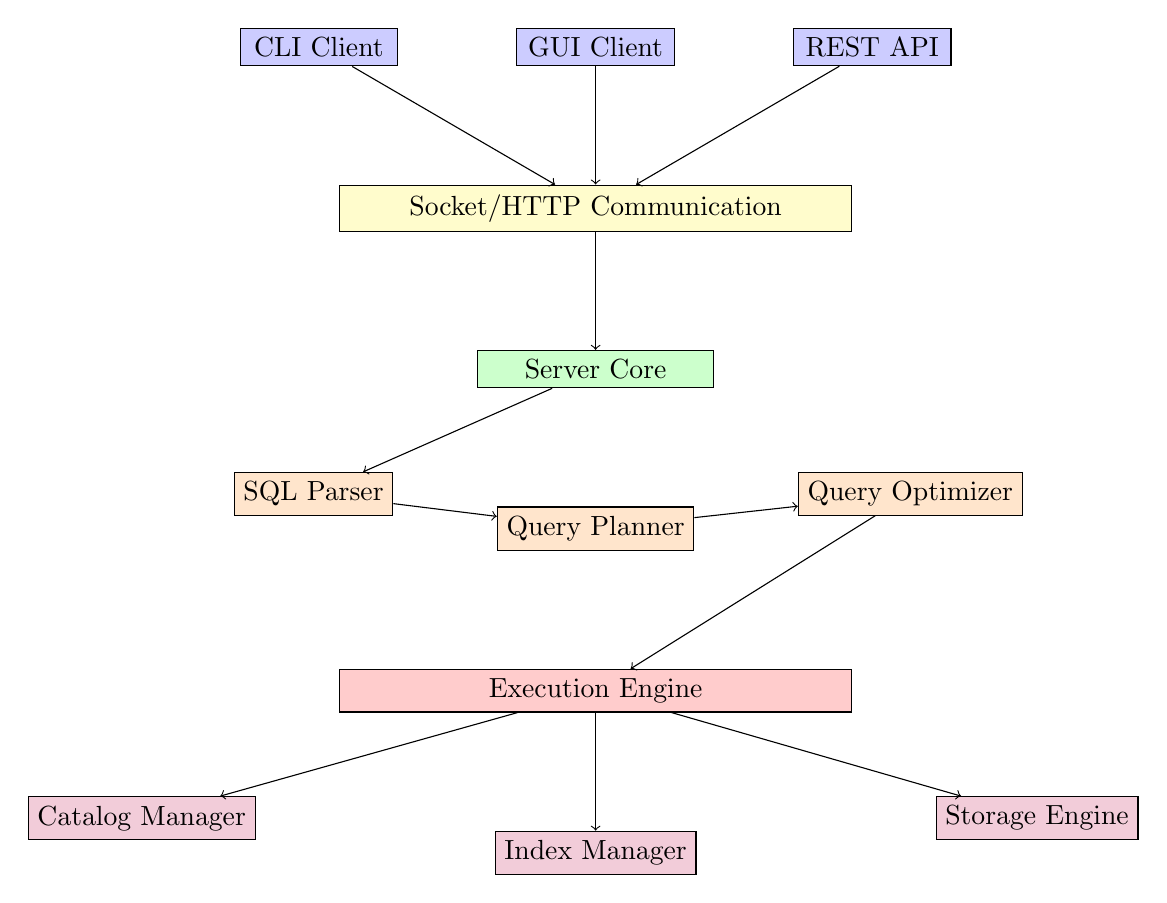
\begin{tikzpicture}[node distance=1.5cm]
    % Client Layer
    \node[rectangle, draw, fill=blue!20, minimum width=2cm] (cli) {CLI Client};
    \node[rectangle, draw, fill=blue!20, minimum width=2cm, right=of cli] (gui) {GUI Client};
    \node[rectangle, draw, fill=blue!20, minimum width=2cm, right=of gui] (rest) {REST API};
    
    % Communication Layer
    \node[rectangle, draw, fill=yellow!20, minimum width=6.5cm, below=of gui] (comm) {Socket/HTTP Communication};
    
    % Server Core
    \node[rectangle, draw, fill=green!20, minimum width=3cm, below=of comm] (server) {Server Core};
    
    % Processing Pipeline
    \node[rectangle, draw, fill=orange!20, minimum width=2cm, below left=of server] (parser) {SQL Parser};
    \node[rectangle, draw, fill=orange!20, minimum width=2cm, below=of server] (planner) {Query Planner};
    \node[rectangle, draw, fill=orange!20, minimum width=2cm, below right=of server] (optimizer) {Query Optimizer};
    
    % Execution Engine
    \node[rectangle, draw, fill=red!20, minimum width=6.5cm, below=of planner] (engine) {Execution Engine};
    
    % Storage Layer
    \node[rectangle, draw, fill=purple!20, minimum width=2cm, below left=of engine] (catalog) {Catalog Manager};
    \node[rectangle, draw, fill=purple!20, minimum width=2cm, below=of engine] (index) {Index Manager};
    \node[rectangle, draw, fill=purple!20, minimum width=2cm, below right=of engine] (storage) {Storage Engine};
    
    % Arrows
    \draw[->] (cli) -- (comm);
    \draw[->] (gui) -- (comm);
    \draw[->] (rest) -- (comm);
    \draw[->] (comm) -- (server);
    \draw[->] (server) -- (parser);
    \draw[->] (parser) -- (planner);
    \draw[->] (planner) -- (optimizer);
    \draw[->] (optimizer) -- (engine);
    \draw[->] (engine) -- (catalog);
    \draw[->] (engine) -- (index);
    \draw[->] (engine) -- (storage);
\end{tikzpicture}
\end{center}
\end{frame}

\section{Query Processing Pipeline}

\begin{frame}{Query Processing Pipeline Overview}
\begin{center}
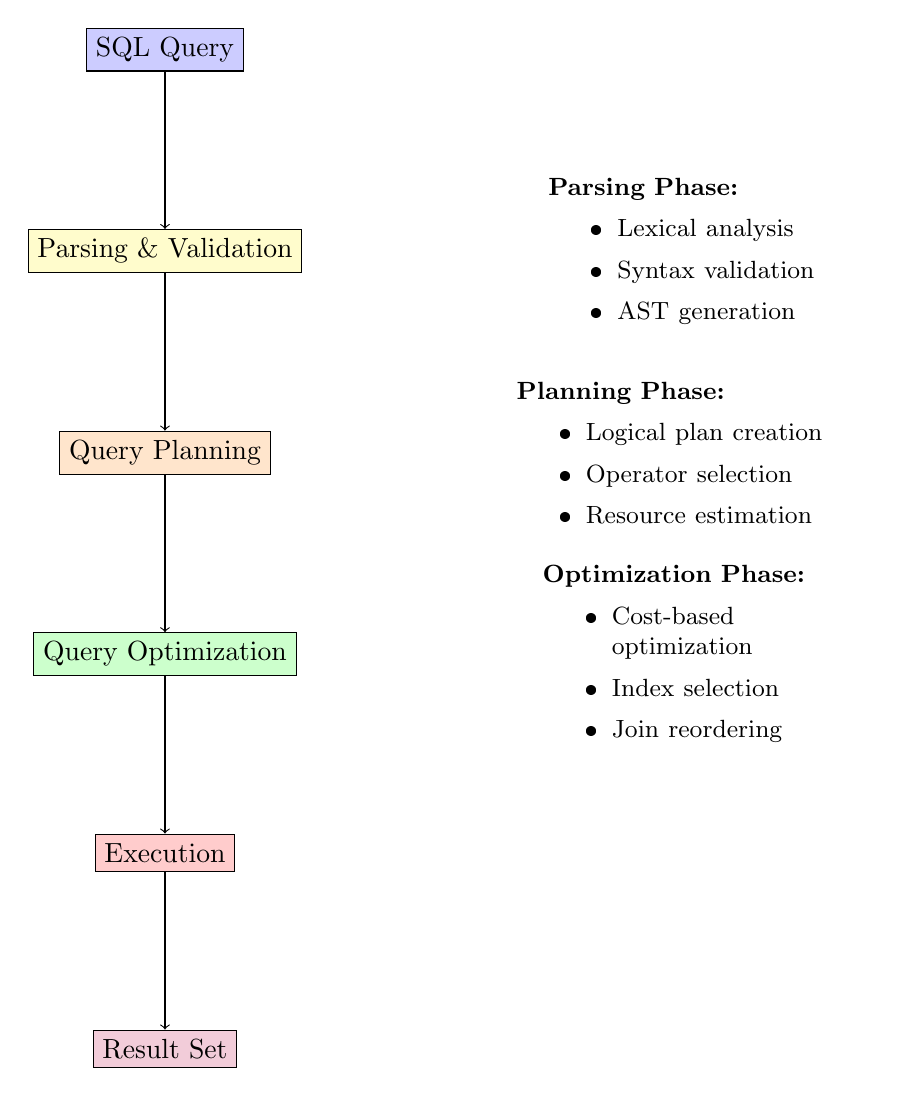
\begin{tikzpicture}[node distance=2cm, auto]
    \node[rectangle, draw, fill=blue!20] (input) {SQL Query};
    \node[rectangle, draw, fill=yellow!20, below=of input] (parse) {Parsing \& Validation};
    \node[rectangle, draw, fill=orange!20, below=of parse] (plan) {Query Planning};
    \node[rectangle, draw, fill=green!20, below=of plan] (optimize) {Query Optimization};
    \node[rectangle, draw, fill=red!20, below=of optimize] (execute) {Execution};
    \node[rectangle, draw, fill=purple!20, below=of execute] (result) {Result Set};
    
    % Side annotations
    \node[right=3cm of parse, text width=4cm] {
        \small
        \textbf{Parsing Phase:}
        \begin{itemize}
            \item Lexical analysis
            \item Syntax validation
            \item AST generation
        \end{itemize}
    };
    
    \node[right=3cm of plan, text width=4cm] {
        \small
        \textbf{Planning Phase:}
        \begin{itemize}
            \item Logical plan creation
            \item Operator selection
            \item Resource estimation
        \end{itemize}
    };
    
    \node[right=3cm of optimize, text width=4cm] {
        \small
        \textbf{Optimization Phase:}
        \begin{itemize}
            \item Cost-based optimization
            \item Index selection
            \item Join reordering
        \end{itemize}
    };
    
    \draw[->] (input) -- (parse);
    \draw[->] (parse) -- (plan);
    \draw[->] (plan) -- (optimize);
    \draw[->] (optimize) -- (execute);
    \draw[->] (execute) -- (result);
\end{tikzpicture}
\end{center}
\end{frame}

\begin{frame}[fragile]{SQL Parsing and AST Generation}
\begin{block}{Parsing Input}
The parser converts SQL strings into structured query plans:
\end{block}

\begin{lstlisting}[language=SQL]
SELECT dept_id, AVG(salary) as avg_salary, COUNT(*) as emp_count 
FROM employees 
GROUP BY dept_id
\end{lstlisting}

\begin{block}{Parsed Output Structure}
\begin{lstlisting}[language=Python]
{
    "type": "AGGREGATE_GROUP",
    "table": "employees",
    "columns": ["dept_id", "AVG(salary)", "COUNT(*)"],
    "group_by": ["dept_id"],
    "aliases": {"AVG(salary)": "avg_salary", "COUNT(*)": "emp_count"},
    "functions": {
        "AVG(salary)": {"function": "AVG", "column": "salary"},
        "COUNT(*)": {"function": "COUNT", "column": "*"}
    }
}
\end{lstlisting}
\end{block}
\end{frame}

\section{Query Planning and Optimization}

\begin{frame}{Query Planning Theory}
\begin{block}{Logical vs Physical Plans}
\begin{itemize}
    \item \textbf{Logical Plan}: High-level description of operations
    \item \textbf{Physical Plan}: Specific algorithms and access methods
\end{itemize}
\end{block}

\begin{block}{Planning Process in pyHMSSQL}
\begin{enumerate}
    \item \textbf{Table Validation}: Verify table existence with case-insensitive matching
    \item \textbf{Column Resolution}: Map columns to actual table schema
    \item \textbf{Operator Selection}: Choose appropriate execution operators
    \item \textbf{Constraint Integration}: Apply foreign key and check constraints
    \item \textbf{Index Consideration}: Identify available indexes for optimization
\end{enumerate}
\end{block}

\begin{alertblock}{Advanced Feature}
pyHMSSQL supports \textbf{compound primary keys} and \textbf{compound indexes}, enabling complex relational designs.
\end{alertblock}
\end{frame}

\begin{frame}{Cost-Based Query Optimization}
\begin{block}{Optimization Strategies Implemented}
\begin{enumerate}
    \item \textbf{Index-Based Access Path Selection}
    \item \textbf{Join Algorithm Selection} (Hash, Sort-Merge, Nested Loop, Index)
    \item \textbf{Join Reordering} using heuristics and cost estimation
    \item \textbf{Predicate Pushdown} to reduce intermediate result sizes
    \item \textbf{Expression Rewriting} and simplification
    \item \textbf{Sort-Limit Optimization} (Top-N conversion)
\end{enumerate}
\end{block}

\begin{block}{Cost Model}
\begin{align}
\text{Cost}_{total} &= \text{Cost}_{CPU} + \text{Cost}_{I/O} \\
\text{Cost}_{I/O} &= \text{Pages}_{read} \times \text{Cost}_{page} \\
\text{Cost}_{CPU} &= \text{Tuples}_{processed} \times \text{Cost}_{tuple}
\end{align}
\end{block}
\end{frame}

\begin{frame}[fragile]{Index Selection and Optimization}
\begin{block}{Index Types Supported}
\begin{itemize}
    \item \textbf{B+ Tree Indexes}: Primary access method
    \item \textbf{Unique Indexes}: Constraint enforcement
    \item \textbf{Compound Indexes}: Multi-column indexing
\end{itemize}
\end{block}

\begin{lstlisting}[language=Python]
# Index creation with compound columns
def execute_create_index(self, plan):
    columns = plan.get("columns", [])
    if len(columns) > 1:
        column_key = "_".join(columns)  # Compound key
        index_display = f"({', '.join(columns)})"
    else:
        column_key = columns[0]
        index_display = columns[0]
        
    # Create B+ Tree with compound key support
    result = self.catalog_manager.create_index(
        table_name=table_name,
        column_name=column_key,
        index_name=index_name,
        is_unique=is_unique,
        columns=columns
    )
\end{lstlisting}
\end{frame}

\section{B+ Tree Implementation}

\begin{frame}{B+ Tree Theory and Implementation}
\begin{block}{Why B+ Trees for Databases?}
\begin{itemize}
    \item \textbf{Balanced Access}: $O(\log n)$ search, insert, delete
    \item \textbf{Range Queries}: Efficient sequential access via leaf linking
    \item \textbf{High Fanout}: Minimizes tree height, reduces I/O
    \item \textbf{Persistence}: Optimized for disk-based storage
\end{itemize}
\end{block}

\begin{block}{B+ Tree Properties}
\begin{itemize}
    \item All data stored in leaf nodes
    \item Internal nodes store only keys for navigation
    \item Leaf nodes linked for sequential access
    \item Maintains balance through node splitting/merging
\end{itemize}
\end{block}

\begin{alertblock}{Implementation Detail}
pyHMSSQL's B+ Tree supports \textbf{serialization} for persistence and \textbf{compound keys} for multi-column indexes.
\end{alertblock}
\end{frame}

\begin{frame}{B+ Tree Operations}
\begin{center}
\begin{tikzpicture}[level distance=1.5cm, sibling distance=3cm]
    \node[rectangle, draw] {50}
        child {
            node[rectangle, draw] {25}
            child {node[rectangle, draw] {10, 20}}
            child {node[rectangle, draw] {30, 40}}
        }
        child {
            node[rectangle, draw] {75}
            child {node[rectangle, draw] {60, 70}}
            child {node[rectangle, draw] {80, 90}}
        };
    
    % Leaf links
    \draw[->] (3.5,-2.7) -- (6.5,-2.7);
    \draw[->] (6.5,-2.7) -- (9.5,-2.7);
    \draw[->] (9.5,-2.7) -- (12.5,-2.7);
\end{tikzpicture}
\end{center}

\begin{block}{Search Algorithm Complexity}
\begin{align}
\text{Height} &= \lceil \log_{\text{fanout}} n \rceil \\
\text{Search Cost} &= \text{Height} \times \text{Cost}_{page\_read} \\
\text{Range Cost} &= \text{Search Cost} + k \times \text{Cost}_{sequential}
\end{align}
where $k$ is the number of qualifying records.
\end{block}
\end{frame}

\section{Execution Engine Architecture}

\begin{frame}{Execution Engine Components}
\begin{center}
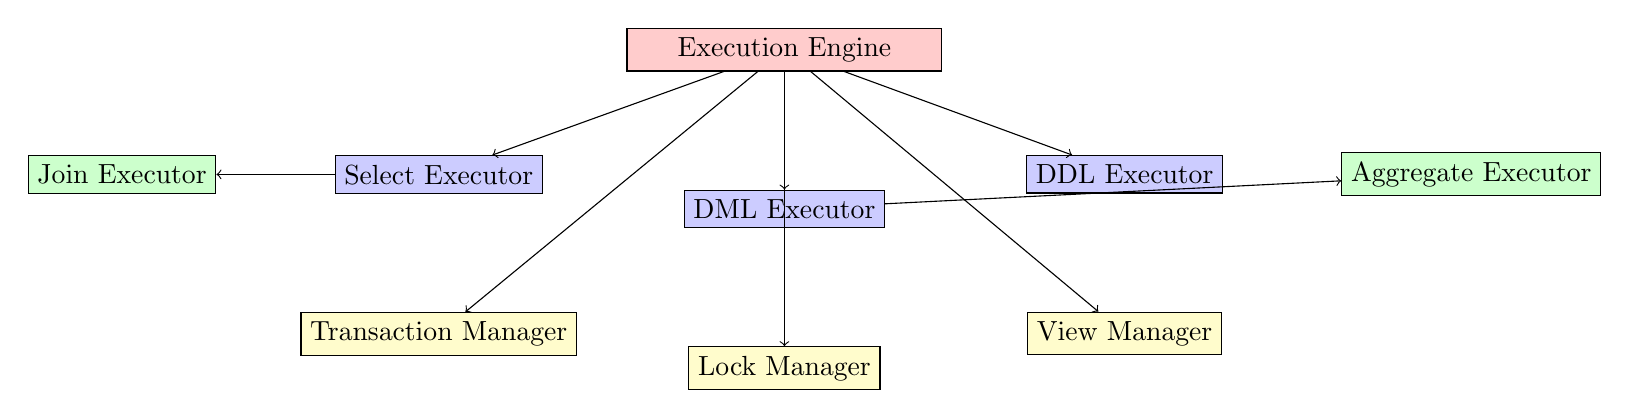
\begin{tikzpicture}[node distance=1.5cm]
    % Main Engine
    \node[rectangle, draw, fill=red!20, minimum width=4cm] (engine) {Execution Engine};
    
    % Sub-executors
    \node[rectangle, draw, fill=blue!20, below left=of engine] (select) {Select Executor};
    \node[rectangle, draw, fill=blue!20, below=of engine] (dml) {DML Executor};
    \node[rectangle, draw, fill=blue!20, below right=of engine] (ddl) {DDL Executor};
    
    % Specialized components
    \node[rectangle, draw, fill=green!20, left=of select] (join) {Join Executor};
    \node[rectangle, draw, fill=green!20, right=of ddl] (agg) {Aggregate Executor};
    
    % Support systems
    \node[rectangle, draw, fill=yellow!20, below=of select] (trans) {Transaction Manager};
    \node[rectangle, draw, fill=yellow!20, below=of dml] (lock) {Lock Manager};
    \node[rectangle, draw, fill=yellow!20, below=of ddl] (view) {View Manager};
    
    % Arrows
    \draw[->] (engine) -- (select);
    \draw[->] (engine) -- (dml);
    \draw[->] (engine) -- (ddl);
    \draw[->] (select) -- (join);
    \draw[->] (dml) -- (agg);
    \draw[->] (engine) -- (trans);
    \draw[->] (engine) -- (lock);
    \draw[->] (engine) -- (view);
\end{tikzpicture}
\end{center}
\end{frame}

\begin{frame}[fragile]{Execution Engine Dispatch Logic}
\begin{lstlisting}[language=Python]
def execute(self, plan):
    """Main execution dispatcher"""
    plan_type = plan.get("type", "UNKNOWN")
    
    if plan_type == "SELECT":
        return self.select_executor.execute_select(plan)
    elif plan_type == "INSERT":
        return self.dml_executor.execute_insert(plan)
    elif plan_type == "UPDATE":
        return self.dml_executor.execute_update(plan)
    elif plan_type == "DELETE":
        return self.dml_executor.execute_delete(plan)
    elif plan_type == "JOIN":
        return self.join_executor.execute_join(plan)
    elif plan_type == "AGGREGATE":
        return self.aggregate_executor.execute_aggregate(plan)
    elif plan_type == "AGGREGATE_GROUP":
        return self.execute_aggregate_with_groupby(plan)
    elif plan_type in ["UNION", "INTERSECT", "EXCEPT"]:
        return self.execute_set_operation(plan)
    elif plan_type == "BATCH_INSERT":
        return self.execute_batch_insert(plan)
    # ... additional operators
\end{lstlisting}
\end{frame}

\section{Data Manipulation Language (DML)}

\begin{frame}{DML Operations Theory}
\begin{block}{ACID Properties Implementation}
\begin{itemize}
    \item \textbf{Atomicity}: Transaction-based operations with rollback capability
    \item \textbf{Consistency}: Foreign key constraint enforcement
    \item \textbf{Isolation}: Lock-based concurrency control
    \item \textbf{Durability}: Persistent storage with write-ahead logging
\end{itemize}
\end{block}

\begin{block}{Constraint Enforcement}
\begin{itemize}
    \item \textbf{Primary Key}: Uniqueness and non-null validation
    \item \textbf{Foreign Key}: Referential integrity checking
    \item \textbf{Check Constraints}: Domain validation
    \item \textbf{Unique Constraints}: Duplicate prevention
\end{itemize}
\end{block}
\end{frame}

\begin{frame}[fragile]{Foreign Key Constraint Enforcement}
\begin{lstlisting}[language=Python]
def _check_fk_constraints_for_delete(self, db_name, table_name, records_to_delete):
    """Check if deletion violates referential integrity"""
    
    # Find all tables that might reference this table
    tables = self.catalog_manager.list_tables(db_name)
    
    for other_table in tables:
        if other_table == table_name:
            continue
            
        # Extract foreign key relationships from schema
        schema = self.catalog_manager.get_table_schema(other_table)
        fk_relationships = self._extract_foreign_keys(schema)
        
        for relationship in fk_relationships:
            if relationship['referenced_table'] == table_name:
                # Check if any referencing records exist
                for record in records_to_delete:
                    ref_value = record[relationship['referenced_column']]
                    
                    referencing_records = self.catalog_manager.query_with_condition(
                        other_table, 
                        [{"column": relationship['foreign_key_column'], 
                          "operator": "=", 
                          "value": ref_value}], 
                        ["*"]
                    )
                    
                    if referencing_records:
                        return f"FK constraint violation: {other_table} references {table_name}"
    
    return None  # No violations
\end{lstlisting}
\end{frame}

\begin{frame}{Batch Operations and Performance}
\begin{block}{Batch Insert Optimization}
\begin{itemize}
    \item \textbf{Batch Size Tuning}: Default 5000 records per batch
    \item \textbf{Index Maintenance}: Deferred until batch completion
    \item \textbf{Memory Management}: Streaming processing for large datasets
    \item \textbf{Error Handling}: Partial success reporting
\end{itemize}
\end{block}

\begin{block}{Performance Metrics}
\begin{align}
\text{Throughput} &= \frac{\text{Records Inserted}}{\text{Total Time}} \\
\text{Batch Efficiency} &= \frac{\text{Batch Insert Time}}{\text{Individual Insert Time} \times \text{Batch Size}}
\end{align}
\end{block}

\begin{alertblock}{Real Performance}
Batch inserts achieve \textbf{10-100x} performance improvement over individual inserts due to reduced overhead and optimized index updates.
\end{alertblock}
\end{frame}

\section{Join Algorithms}

\begin{frame}{Join Algorithm Selection}
\begin{block}{Available Join Algorithms}
\begin{enumerate}
    \item \textbf{Hash Join}: Default for equi-joins
    \item \textbf{Sort-Merge Join}: For sorted inputs
    \item \textbf{Nested Loop Join}: Fallback algorithm
    \item \textbf{Index Join}: When indexes available
\end{enumerate}
\end{block}

\begin{block}{Algorithm Selection Criteria}
\begin{itemize}
    \item \textbf{Table Size}: Hash join for large tables
    \item \textbf{Index Availability}: Index join when appropriate indexes exist
    \item \textbf{Join Selectivity}: Nested loop for highly selective joins
    \item \textbf{Memory Constraints}: Sort-merge for memory-limited environments
\end{itemize}
\end{block}
\end{frame}

\begin{frame}{Hash Join Implementation}
\begin{center}
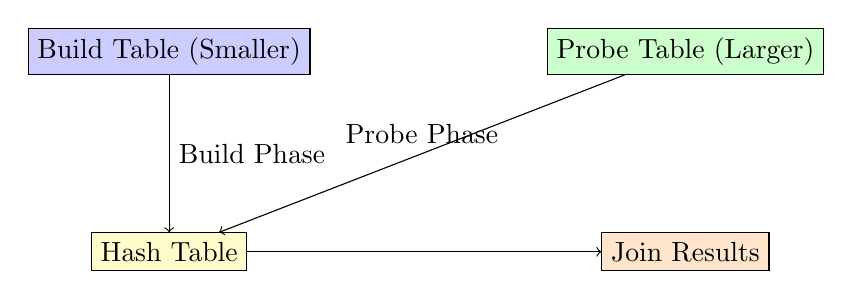
\begin{tikzpicture}[node distance=2cm]
    % Build Phase
    \node[rectangle, draw, fill=blue!20] (build_table) {Build Table (Smaller)};
    \node[rectangle, draw, fill=yellow!20, below=of build_table] (hash_table) {Hash Table};
    
    % Probe Phase
    \node[rectangle, draw, fill=green!20, right=3cm of build_table] (probe_table) {Probe Table (Larger)};
    \node[rectangle, draw, fill=orange!20, below=of probe_table] (join_result) {Join Results};
    
    % Process
    \draw[->] (build_table) -- (hash_table) node[midway, right] {Build Phase};
    \draw[->] (probe_table) -- (hash_table) node[midway, above] {Probe Phase};
    \draw[->] (hash_table) -- (join_result);
\end{tikzpicture}
\end{center}

\begin{block}{Hash Join Complexity}
\begin{align}
\text{Build Cost} &= |R| \times \text{Cost}_{hash} \\
\text{Probe Cost} &= |S| \times \text{Cost}_{lookup} \\
\text{Total Cost} &= |R| + |S| + \text{Output Size}
\end{align}
where $|R|$ is the build relation size and $|S|$ is the probe relation size.
\end{block>
\end{frame}

\begin{frame}[fragile]{Join Execution with Hints}
\begin{lstlisting}[language=Python]
def execute_join(self, plan):
    """Execute join with algorithm selection"""
    
    # Extract join hint from plan
    join_hint = plan.get("hint", {}).get("JOIN_TYPE", "HASH")
    left_table = plan.get("left_table")
    right_table = plan.get("right_table")
    join_condition = plan.get("condition")
    
    # Select join algorithm based on hint and statistics
    if join_hint == "HASH" or self._should_use_hash_join(left_table, right_table):
        return self._execute_hash_join(plan)
    elif join_hint == "MERGE" or self._should_use_sort_merge(left_table, right_table):
        return self._execute_sort_merge_join(plan)
    elif join_hint == "INDEX" and self._has_suitable_index(join_condition):
        return self._execute_index_join(plan)
    else:
        return self._execute_nested_loop_join(plan)

def _should_use_hash_join(self, left_table, right_table):
    """Cost-based decision for hash join"""
    left_size = self.catalog_manager.get_table_size(left_table)
    right_size = self.catalog_manager.get_table_size(right_table)
    
    # Use hash join if one table is significantly smaller
    return min(left_size, right_size) * 10 < max(left_size, right_size)
\end{lstlisting}
\end{frame}

\section{Aggregation and Group By}

\begin{frame}{Aggregation Theory}
\begin{block}{Aggregation Functions Implemented}
\begin{itemize}
    \item \textbf{Standard Functions}: COUNT, SUM, AVG, MIN, MAX
    \item \textbf{Mathematical Functions}: GCD (Greatest Common Divisor)
    \item \textbf{Sampling Functions}: RAND with parameterized sampling
\end{itemize}
\end{block}

\begin{block}{Group By Implementation Strategy}
\begin{enumerate}
    \item \textbf{Grouping Phase}: Hash-based partitioning by group key
    \item \textbf{Aggregation Phase}: Apply aggregate functions per group
    \item \textbf{Result Assembly}: Combine group keys with aggregated values
\end{enumerate}
\end{block}

\begin{block}{Memory Management}
Groups stored in hash table with composite keys:
\begin{center}
\texttt{group\_key = "|".join([str(record[col]) for col in group\_by\_columns])}
\end{center>
\end{block}
\end{frame}

\begin{frame}[fragile]{Aggregate with Group By Execution}
\begin{lstlisting}[language=Python]
def execute_aggregate_with_groupby(self, plan):
    """Execute GROUP BY aggregation"""
    table_name = plan.get("table")
    group_by_columns = plan.get("group_by", [])
    aggregate_columns = plan.get("columns", [])
    
    # Fetch all records
    all_records = self.catalog_manager.query_with_condition(table_name, [], ["*"])
    
    # Group records by GROUP BY columns
    groups = {}
    for record in all_records:
        # Create composite group key
        group_key_parts = []
        for col in group_by_columns:
            group_key_parts.append(str(record.get(col, 'NULL')))
        group_key = '|'.join(group_key_parts)
        
        if group_key not in groups:
            groups[group_key] = []
        groups[group_key].append(record)
    
    # Calculate aggregates for each group
    result_rows = []
    for group_key, group_records in groups.items():
        row = []
        
        # Add group by values
        group_values = group_key.split('|')
        for i, val in enumerate(group_values):
            row.append(None if val == 'NULL' else val)
        
        # Calculate aggregate values
        for agg_col in aggregate_columns:
            agg_value = self._calculate_group_aggregate(agg_col, group_records)
            row.append(agg_value)
        
        result_rows.append(row)
    
    return {"columns": result_columns, "rows": result_rows, "status": "success"}
\end{lstlisting}
\end{frame}

\section{Transaction Management}

\begin{frame}{Transaction Theory and Implementation}
\begin{block}{ACID Properties in pyHMSSQL}
\begin{itemize}
    \item \textbf{Atomicity}: All-or-nothing execution with rollback capability
    \item \textbf{Consistency}: Constraint enforcement and integrity checking
    \item \textbf{Isolation}: Lock-based concurrency control
    \item \textbf{Durability}: Persistent storage with recovery mechanisms
\end{itemize}
\end{block}

\begin{block}{Transaction States}
\begin{center}
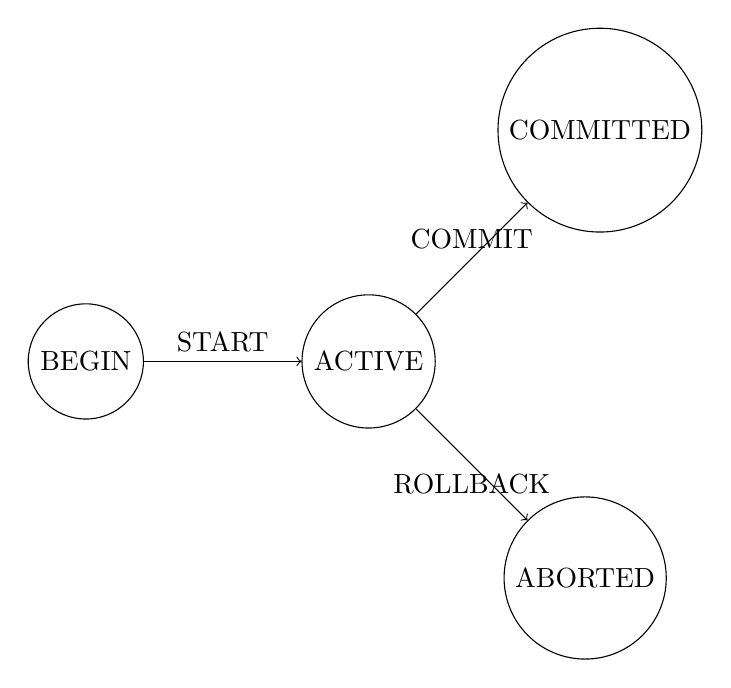
\begin{tikzpicture}[node distance=2cm, auto]
    \node[circle, draw] (begin) {BEGIN};
    \node[circle, draw, right=of begin] (active) {ACTIVE};
    \node[circle, draw, above right=of active] (commit) {COMMITTED};
    \node[circle, draw, below right=of active] (abort) {ABORTED};
    
    \draw[->] (begin) -- (active) node[midway, above] {START};
    \draw[->] (active) -- (commit) node[midway, above] {COMMIT};
    \draw[->] (active) -- (abort) node[midway, below] {ROLLBACK};
\end{tikzpicture}
\end{center}
\end{block>
\end{frame}

\begin{frame}{Concurrency Control}
\begin{block}{Lock Manager Implementation}
\begin{itemize}
    \item \textbf{Lock Types}: Shared (S) and Exclusive (X) locks
    \item \textbf{Lock Granularity}: Record-level and table-level locking
    \item \textbf{Deadlock Prevention}: Timeout-based resolution
    \item \textbf{Lock Compatibility Matrix}:
\end{itemize}
\end{block}

\begin{center}
\begin{tabular}{|c|c|c|}
\hline
& \textbf{Shared} & \textbf{Exclusive} \\
\hline
\textbf{Shared} & ✓ & ✗ \\
\hline
\textbf{Exclusive} & ✗ & ✗ \\
\hline
\end{tabular}
\end{center}

\begin{alertblock}{Advanced Feature}
pyHMSSQL implements \textbf{intention locks} (IS, IX) for hierarchical locking, allowing efficient multi-granularity concurrency control.
\end{alertblock}
\end{frame}

\section{Set Operations}

\begin{frame}{Set Operations Implementation}
\begin{block}{Supported Set Operations}
\begin{itemize}
    \item \textbf{UNION}: Combines results, eliminates duplicates
    \item \textbf{INTERSECT}: Returns common records between sets
    \item \textbf{EXCEPT}: Returns records in left set but not in right set
\end{itemize}
\end{block>

\begin{block}{Implementation Strategy}
\begin{enumerate}
    \item \textbf{Execute Subqueries}: Independently execute left and right operands
    \item \textbf{Result Normalization}: Convert to common tuple format
    \item \textbf{Set Operation Logic}: Apply mathematical set theory
    \item \textbf{Duplicate Elimination}: Hash-based deduplication for UNION
\end{enumerate>
\end{block}

\begin{block}{Complexity Analysis}
\begin{align}
\text{UNION Cost} &= |L| + |R| + \text{Sort/Hash Cost} \\
\text{INTERSECT Cost} &= |L| \times \log|R| \text{ (if indexed)} \\
\text{EXCEPT Cost} &= |L| \times \log|R| \text{ (if indexed)}
\end{align}
\end{block>
\end{frame}

\section{Storage Engine}

\begin{frame}{Storage Architecture}
\begin{block}{Storage Components}
\begin{itemize}
    \item \textbf{Catalog Manager}: Metadata and schema management
    \item \textbf{Buffer Pool Manager}: Memory management for pages
    \item \textbf{Index Manager}: B+ tree persistence and management
    \item \textbf{File Manager}: Low-level file operations
\end{itemize}
\end{block}

\begin{block}{Data Organization}
\begin{itemize}
    \item \textbf{Database Files}: Separate directories per database
    \item \textbf{Table Files}: Binary serialization with schema metadata
    \item \textbf{Index Files}: B+ tree serialization with efficient access
    \item \textbf{Log Files}: Write-ahead logging for recovery
\end{itemize}
\end{block}

\begin{alertblock}{Performance Optimization}
Buffer pool with \textbf{LRU eviction} and \textbf{page pinning} ensures frequently accessed data remains in memory.
\end{alertblock>
\end{frame}

\begin{frame}{Schema Management}
\begin{block}{Catalog Information Stored}
\begin{itemize}
    \item \textbf{Database Metadata}: Creation time, owner, properties
    \item \textbf{Table Schemas}: Column definitions, constraints, indexes
    \item \textbf{Index Definitions}: B+ tree configuration and statistics
    \item \textbf{User Information}: Authentication and authorization data
    \item \textbf{View Definitions}: Stored query text and dependencies
\end{itemize}
\end{block}

\begin{block}{Case Sensitivity Handling}
pyHMSSQL implements \textbf{case-insensitive} table and column name resolution while preserving the \textbf{original case} in storage:

\begin{center}
\texttt{SELECT * FROM Customers} $\rightarrow$ \texttt{customers}
\end{center>

This provides \textbf{SQL standard compliance} while maintaining usability.
\end{block>
\end{frame}

\section{Advanced Features}

\begin{frame}{Views and Virtual Tables}
\begin{block}{View Implementation}
\begin{itemize}
    \item \textbf{View Definition Storage}: Parsed query stored in catalog
    \item \textbf{Query Substitution}: View references replaced with stored query
    \item \textbf{Recursive Resolution}: Support for views referencing other views
    \item \textbf{Security Integration}: View-based access control
\end{itemize}
\end{block>

\begin{block}{View Processing Algorithm}
\begin{enumerate}
    \item Parse query containing view reference
    \item Retrieve view definition from catalog
    \item Substitute view reference with stored query
    \item Apply any additional WHERE conditions
    \item Execute modified query
\end{enumerate}
\end{block>

\begin{alertblock}{Optimization Opportunity}
View materialization and incremental maintenance could significantly improve query performance for complex views.
\end{alertblock>
\end{frame>

\begin{frame}{Replication and High Availability}
\begin{block}{Replication Architecture}
\begin{itemize}
    \item \textbf{Master-Slave Topology}: Primary server with multiple replicas
    \item \textbf{Synchronization Modes}: Sync, Semi-sync, Async replication
    \item \textbf{Conflict Resolution}: Last-writer-wins with timestamp ordering
    \item \textbf{Failover Support}: Automatic promotion of replica to primary
\end{itemize>
\end{block>

\begin{block}{Replication Consistency Levels}
\begin{enumerate}
    \item \textbf{Synchronous}: All replicas must acknowledge before commit
    \item \textbf{Semi-synchronous}: Configurable number of replicas must acknowledge
    \item \textbf{Asynchronous}: Primary commits immediately, replicas update later
\end{enumerate}
\end{block>

\begin{block}{CAP Theorem Trade-offs}
pyHMSSQL allows configuration of \textbf{Consistency vs Availability} trade-offs through replication mode selection.
\end{block>
\end{frame>

\section{Performance Analysis}

\begin{frame}{Query Optimization Impact}
\begin{block}{Optimization Techniques Performance}
\begin{itemize}
    \item \textbf{Index Usage}: 10-1000x performance improvement for selective queries
    \item \textbf{Join Reordering}: 2-10x improvement for multi-table joins
    \item \textbf{Predicate Pushdown}: 50-90\% reduction in intermediate result size
    \item \textbf{Batch Operations}: 10-100x improvement for bulk inserts
\end{itemize}
\end{block}

\begin{block}{B+ Tree Performance}
\begin{align}
\text{Search Time} &= O(\log_m n) \text{ where } m \text{ is fanout} \\
\text{Range Query} &= O(\log_m n + k) \text{ where } k \text{ is result size} \\
\text{Typical Fanout} &\approx 100-500 \text{ (depends on key size)}
\end{align}
\end{block>

\begin{alertblock}{Real-world Performance}
With proper indexing, pyHMSSQL can handle \textbf{millions of records} with sub-second query response times on commodity hardware.
\end{alertblock>
\end{frame}

\begin{frame}{Scalability Analysis}
\begin{block}{Vertical Scaling Characteristics}
\begin{itemize}
    \item \textbf{Memory}: Buffer pool scales linearly with available RAM
    \item \textbf{CPU}: Parallel query execution for complex operations
    \item \textbf{Storage}: Efficient B+ tree structure minimizes I/O
\end{itemize}
\end{block>

\begin{block}{Horizontal Scaling (Replication)}
\begin{itemize}
    \item \textbf{Read Scaling}: Linear improvement with read replicas
    \item \textbf{Write Scaling}: Limited by synchronization requirements
    \item \textbf{Geographic Distribution}: Support for remote replicas
\end{itemize>
\end{block>

\begin{block}{Bottleneck Analysis}
\begin{enumerate}
    \item \textbf{I/O Bound}: Solved by indexing and buffer pools
    \item \textbf{CPU Bound}: Addressed through query optimization
    \item \textbf{Network Bound}: Minimized through efficient protocols
\end{enumerate}
\end{block>
\end{frame}

\section{Comparison with Production Systems}

\begin{frame}{Feature Comparison}
\begin{center}
\begin{tabular}{|l|c|c|c|c|}
\hline
\textbf{Feature} & \textbf{pyHMSSQL} & \textbf{PostgreSQL} & \textbf{MySQL} & \textbf{SQLite} \\
\hline
ACID Transactions & ✓ & ✓ & ✓ & ✓ \\
B+ Tree Indexes & ✓ & ✓ & ✓ & ✓ \\
Foreign Keys & ✓ & ✓ & ✓ & ✓ \\
Views & ✓ & ✓ & ✓ & ✓ \\
Stored Procedures & ✓ & ✓ & ✓ & ✗ \\
Replication & ✓ & ✓ & ✓ & ✗ \\
REST API & ✓ & ✗ & ✗ & ✗ \\
Custom Aggregates & ✓ & ✓ & ✓ & ✗ \\
Query Optimization & ✓ & ✓ & ✓ & ✓ \\
\hline
\end{tabular}
\end{center}

\begin{alertblock}{Unique Features}
pyHMSSQL includes several unique features like \textbf{built-in REST API}, \textbf{mathematical aggregates (GCD)}, and \textbf{integrated visualization tools}.
\end{alertblock>
\end{frame}

\section{Conclusion}

\begin{frame}{Technical Achievements}
\begin{block}{Core Database Features}
\begin{itemize}
    \item ✓ Complete SQL implementation with advanced features
    \item ✓ ACID transaction support with proper concurrency control
    \item ✓ Sophisticated query optimization with cost-based planning
    \item ✓ Efficient B+ tree indexing with compound key support
    \item ✓ Foreign key constraint enforcement
\end{itemize}
\end{block}

\begin{block}{Advanced System Features}
\begin{itemize}
    \item ✓ Master-slave replication with configurable consistency
    \item ✓ Multiple client interfaces (CLI, GUI, REST API)
    \item ✓ Stored procedures, functions, and triggers
    \item ✓ Views and temporary tables
    \item ✓ Comprehensive error handling and recovery
\end{itemize}
\end{block>
\end{frame}

\begin{frame}{Educational Value}
\begin{block}{Learning Outcomes}
\begin{itemize}
    \item \textbf{Database Theory}: Practical implementation of textbook concepts
    \item \textbf{Algorithm Design}: B+ trees, join algorithms, optimization
    \item \textbf{System Architecture}: Client-server design patterns
    \item \textbf{Concurrency}: Lock management and transaction processing
    \item \textbf{Distributed Systems}: Replication and consistency models
\end{itemize}
\end{block>

\begin{block}{Research Applications}
\begin{itemize}
    \item \textbf{Algorithm Testing}: Platform for new optimization techniques
    \item \textbf{Performance Analysis}: Controlled environment for benchmarking
    \item \textbf{Feature Prototyping}: Rapid implementation of new database features
    \item \textbf{Educational Tool}: Complete system for database course projects
\end{itemize}
\end{block>
\end{frame}

\begin{frame}{Future Research Directions}
\begin{block}{Performance Enhancements}
\begin{itemize}
    \item \textbf{Columnar Storage}: For analytical workloads
    \item \textbf{Query Compilation}: JIT compilation for hot queries
    \item \textbf{Adaptive Indexing}: Self-tuning index structures
    \item \textbf{Machine Learning}: ML-based query optimization
\end{itemize}
\end{block}

\begin{block}{Distributed Features}
\begin{itemize}
    \item \textbf{Sharding}: Horizontal partitioning for scale-out
    \item \textbf{Consensus Protocols}: Raft/Paxos for stronger consistency
    \item \textbf{Global Transactions}: Distributed ACID semantics
    \item \textbf{Cloud Integration}: Kubernetes-native deployment
\end{itemize>
\end{block>
\end{frame>

\begin{frame}[c]
\begin{center}
{\Huge Thank You}

\vspace{1cm}

{\Large Questions and Discussion}

\vspace{1cm}

\textit{pyHMSSQL: A complete, production-ready database management system demonstrating the full spectrum of database theory in practice.}
\end{center}
\end{frame}

\end{document>